\chapter{Introduction}

\section{electron dynamics in solids}

\section{attosecond transient absorption spectroscopy (ATAS)}



general description of ATAS

\section{high harmonic generation}

\subsection{three-step model}

\begin{figure}
	\centering
	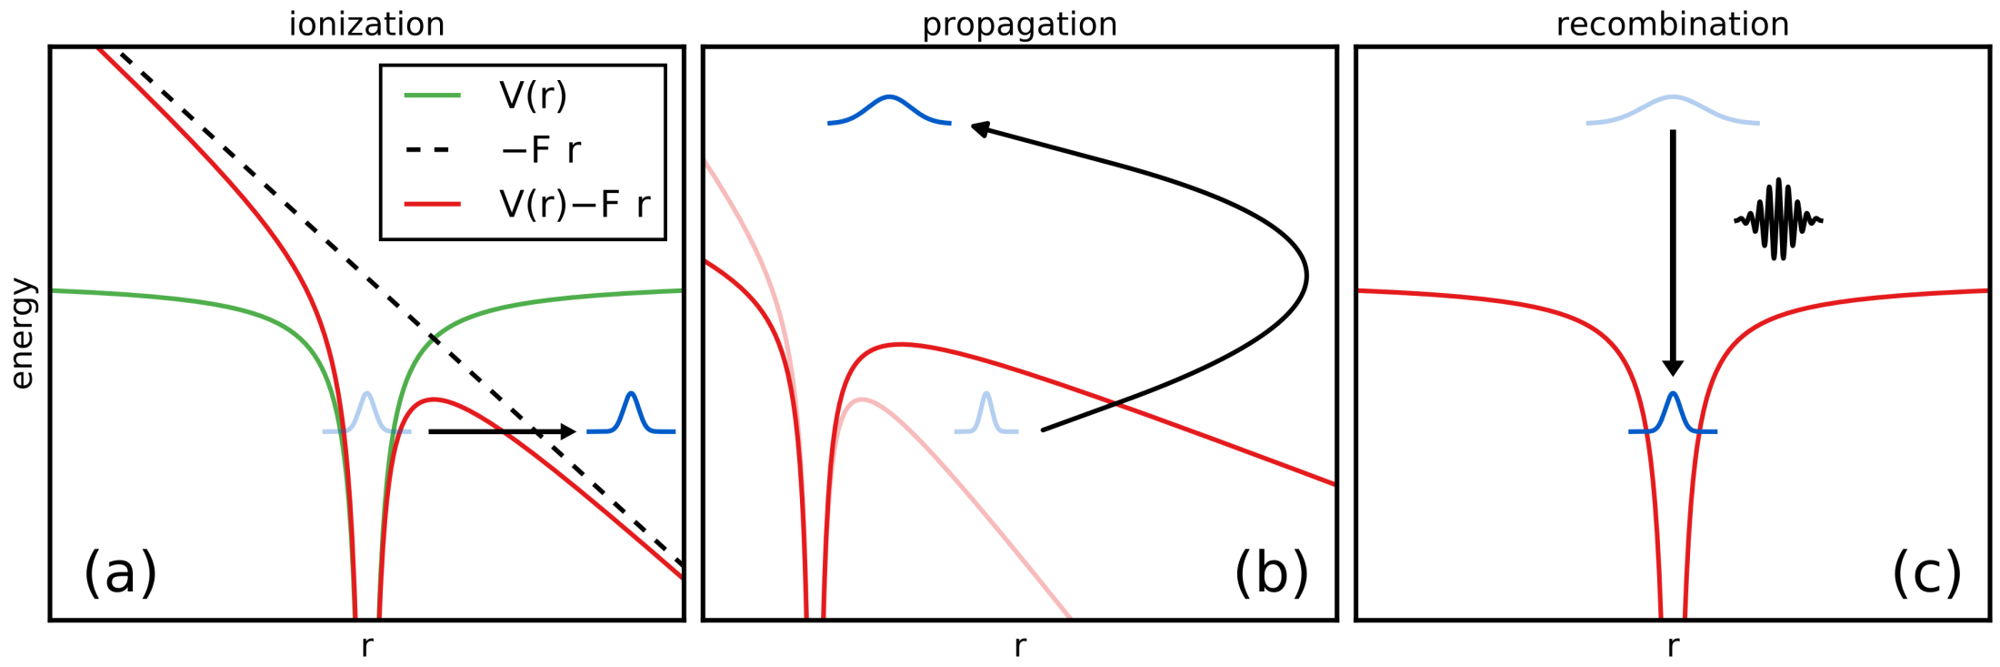
\includegraphics[width=0.75\textwidth]{figures/chap1/ThreeStepModel.png}
	\caption{3 step model from S. Schoun's thesis\cite{schounAttosecondHighHarmonicSpectroscopy2015}.}
	\label{fig:ThreeStepModel}
\end{figure}

single atom response

cycle-averaged quiver energy

\begin{equation}
U_p = \frac{q_e^2 F_0^2}{4 m_e \omega^2} \propto I_0 \lambda^2
\label{eqn:Up}
\end{equation}

cutoff energy:

\begin{equation}
\omega_{cutoff} = I_p + 3.17 U_p
\label{eqn:cutoff}
\end{equation}

semi-classical three step model


\subsection{phase matching}

macroscopic response

things i need to talk about: 

\begin{equation}
\Delta k = \Delta k_{atomic} + \Delta k_{plasma} + \Delta k_{Gouy} + \Delta k_{dipole}
\end{equation}

\subsubsection{1D phase matching model}

for the $q^{th}$ harmonic, the number $N_{out}$ of photons emitted on axis per unit time and of area is proportional to \cite{constantOptimizingHighHarmonic1999}:

\begin{equation}
\rho^2 A_q^2 \frac{4L_{abs}^2}{1+4\pi^2(L_{abs}^2 / L_{coh}^2)} \left[ 1 + \exp\left(-\frac{L_{med}}{L_{abs}}\right) - 2 \exp\left(\frac{\pi L_{med}}{L_{coh}}\right) \exp\left(-\frac{L_{med}}{2L_{abs}}\right) \right]
\label{eqn:HHGNout}
\end{equation}

where $L_{coh} = \pi/\Delta k$ is the coherence length ($\Delta k = k_q - q k_0$)


- critical phase matching pressure (kazamias?)